\chapter{Tree}

\subsubsection{500以上的题目暂时未录入}

\section{Maximum Depth of Binary Tree} %%%%%%%%%%%%%%%%%%%%%%

\subsubsection{Description}

Given a binary tree, find its maximum depth.

The maximum depth is the number of nodes along the longest path from the root node down to the farthest leaf node.

\subsubsection{Solution}

\begin{Code}
private int maxDepth(TreeNode node) {
    if (node == null) {
        return 0;
    }
    return Math.max(maxDepth(node.left), maxDepth(node.right)) + 1;
}
\end{Code}

\newpage

\section{Invert Binary Tree} %%%%%%%%%%%%%%%%%%%%%%

\subsubsection{Description}

Invert a binary tree.
\begin{Code}
     4                              4
   /   \                          /   \
  2     7           to           7     2
 / \   / \                      / \   / \
1   3 6   9                    9   6 3   1
\end{Code}

\subsubsection{Solution I}

\begin{Code}
public TreeNode invertTree(TreeNode root) {
    if (root == null) {
        return null;
    }

    TreeNode right = root.right;
    root.right = invertTree(root.left);
    root.left = invertTree(right);
    return root;
}
\end{Code}

\subsubsection{Solution II}

\begin{Code}
public TreeNode invertTree(TreeNode root) {
    if (root == null) {
        return null;
    }

    Queue<TreeNode> queue = new LinkedList<TreeNode>();
    queue.offer(root);

    while (!queue.isEmpty()) {
        TreeNode node = queue.poll();

        TreeNode left = node.left;
        node.left = node.right;
        node.right = left;

        if (node.left != null) {
            queue.offer(node.left);
        }

        if (node.right != null) {
            queue.offer(node.right);
        }
    }

    return root;
}
\end{Code}

\newpage

\section{Same Tree} %%%%%%%%%%%%%%%%%%%%%%

\subsubsection{Description}

Given two binary trees, write a function to check if they are equal or not.

Two binary trees are considered equal if they are structurally identical and the nodes have the same value.

\subsubsection{Solution}

\begin{Code}
public boolean isSameTree(TreeNode p, TreeNode q) {
    if (p == null && q == null) {
        return true;
    }
    if (p == null || q == null) {
        return false;
    }
    return p.val == q.val && isSameTree(p.left, q.left) && isSameTree(p.right, q.right);
}
\end{Code}

\newpage

\section{Binary Search Tree Iterator} %%%%%%%%%%%%%%%%%%%%%%

\subsubsection{Description}

Implement an iterator over a binary search tree (BST). Your iterator will be initialized with the root node of a BST.

Calling next() will return the next smallest number in the BST.

\textbf{Note:}

next() and hasNext() should run in average O(1) time and uses O(h) memory, where h is the height of the tree.

\subsubsection{Solution}

\begin{Code}
public class BSTIterator {

    private Stack<TreeNode> mStack;
    private TreeNode mCurNode;

    public BSTIterator(TreeNode root) {
        mStack = new Stack<TreeNode>();
        mCurNode = root;
    }

    public boolean hasNext() {
        return !mStack.isEmpty() || mCurNode != null;
    }

    public int next() {
        int result = -1;

        while (hasNext()) {
            if (mCurNode != null) {
                mStack.push(mCurNode);
                mCurNode = mCurNode.left;
            } else {
                mCurNode = mStack.pop();
                result = mCurNode.val;
                mCurNode = mCurNode.right;
                break;
            }
        }

        return result;
    }
}
\end{Code}

\newpage

\section{Lowest Common Ancestor of a Binary Search Tree} %%%%%%%%%%%%%%%%%%%%%%

\subsubsection{Description}

Given a binary search tree (BST), find the lowest common ancestor (LCA) of two given nodes in the BST.

According to the definition of LCA on Wikipedia: “The lowest common ancestor is defined between two nodes v and w as the lowest node in T that has both v and w as descendants (where we allow a node to be a descendant of itself).”
\begin{Code}
        _______6______
       /              \
    ___2__          ___8__
   /      \        /      \
   0      _4       7       9
         /  \
         3   5
\end{Code}
For example, the lowest common ancestor (LCA) of nodes 2 and 8 is 6. Another example is LCA of nodes 2 and 4 is 2, since a node can be a descendant of itself according to the LCA definition.

\subsubsection{Solution}

\begin{Code}
// 耗时9ms
public TreeNode lowestCommonAncestor(TreeNode root, TreeNode p, TreeNode q) {
    if (!checkExist(root, p) || !checkExist(root, q)) {
        throw new IllegalArgumentException("Not exist!!");
    }

    while (root != null) {
        if (p.val < root.val && q.val < root.val) {
            root = root.left;
        } else if (p.val > root.val && q.val > root.val) {
            root = root.right;
        } else {
            break;
        }
    }
    return root;
}

/**
 * 如何判断p或q一定存在,如果是BST就很简单
 */
private boolean checkExist(TreeNode root, TreeNode node) {
    TreeNode cur = root;
    while (cur != null) {
        if (node.val > cur.val) {
            cur = cur.right;
        } else if (node.val < cur.val) {
            cur = cur.left;
        } else {
            return true;
        }
    }
    return false;
}
\end{Code}

\newpage

\section{Balanced Binary Tree} %%%%%%%%%%%%%%%%%%%%%%

\subsubsection{Description}

Given a binary tree, determine if it is height-balanced.

For this problem, a height-balanced binary tree is defined as a binary tree in which the depth of the two subtrees of every node never differ by more than 1.

\subsubsection{Solution}

\begin{Code}
public boolean isBalanced(TreeNode root) {
    return isBalanced(root, null);
}

private boolean isBalanced(TreeNode root, int[] height) {
    if (root == null) {
        return true;
    }

    int[] left = new int[1], right = new int[1];

    boolean result = isBalanced(root.left, left) && isBalanced(root.right, right);

    if (height != null) {
        height[0] = Math.max(left[0], right[0]) + 1;
    }

    return result && Math.abs(left[0] - right[0]) <= 1;
}
\end{Code}

\newpage

\section{Binary Tree Maximum Path Sum} %%%%%%%%%%%%%%%%%%%%%%

\subsubsection{Description}

Given a binary tree, find the maximum path sum.

For this problem, a path is defined as any sequence of nodes from some starting node to any node in the tree along the parent-child connections. The path must contain at least one node and does not need to go through the root.

For example:

Given the below binary tree,
\begin{Code}
       1
      / \
     2   3
\end{Code}

Return 6.

\subsubsection{Solution}

\begin{Code}
public int maxPathSum(TreeNode root) {
    return maxPathSum(root, null);
}

/**
 * max表示包含root的单边路径最大和
 */
private int maxPathSum(TreeNode root, int[] max) {
    if (root == null) {
        return Integer.MIN_VALUE;  // 此处容易错
    }
    int[] left = new int[1], right = new int[1];
    int leftMax = maxPathSum(root.left, left);
    int rightMax = maxPathSum(root.right, right);
    if (max != null) {
        // 三种情况:root, root+left, root+right
        max[0] = max(left[0], right[0], 0) + root.val;
    }

    // 容易错,要考虑到所有可能的情况
    // 左边里面的,右边里面的,光root的,左中右,左中,中右
    return max(leftMax, rightMax, root.val, left[0] + right[0] + root.val,
            left[0] + root.val, right[0] + root.val);
}

private int max(int... vals) {
    int max = Integer.MIN_VALUE;
    for (int val : vals) {
        max = Math.max(max, val);
    }
    return max;
}
\end{Code}

\newpage

\section{Populating Next Right Pointers in Each Node} %%%%%%%%%%%%%%%%%%%%%%

\subsubsection{Description}

Given a binary tree
\begin{Code}
    struct TreeLinkNode {
      TreeLinkNode *left;
      TreeLinkNode *right;
      TreeLinkNode *next;
    }
\end{Code}

Populate each next pointer to point to its next right node. If there is no next right node, the next pointer should be set to NULL.

Initially, all next pointers are set to NULL.

\textbf{Note:}

You may only use constant extra space.

You may assume that it is a perfect binary tree (ie, all leaves are at the same level, and every parent has two children).

For example,

Given the following perfect binary tree,
\begin{Code}
         1
       /  \
      2    3
     / \  / \
    4  5  6  7
\end{Code}

After calling your function, the tree should look like:
\begin{Code}
         1 -> NULL
       /  \
      2 -> 3 -> NULL
     / \  / \
    4->5->6->7 -> NULL
\end{Code}

\newpage

\subsubsection{Solution I}

\begin{Code}
/** 递归法,巧妙地运用dummy使代码很简洁
 *  假定当前root所在层已连好,要连下一层
 */
public void connect(TreeLinkNode root) {
    if (root == null) {
        return;
    }
    TreeLinkNode dummy = new TreeLinkNode(0), cur = dummy;
    for (TreeLinkNode p = root; p != null; p = p.next) {
        if (p.left != null) {
            cur.next = p.left;
            cur = cur.next;
        }
        if (p.right != null) {
            cur.next = p.right;
            cur = cur.next;
        }
    }
    connect(dummy.next);
}

\end{Code}

\subsubsection{Solution II}

\begin{Code}
/**
 * 将递归转成非递归很简单,就加一层循环,且结尾处加root = dummy.next即可
 */
public void connect2(TreeLinkNode root) {
    while (root != null) {
        TreeLinkNode dummy = new TreeLinkNode(0), cur = dummy;

        for (TreeLinkNode p = root; p != null; p = p.next) {
            if (p.left != null) {
                cur.next = p.left;
                cur = cur.next;
            }
            if (p.right != null) {
                cur.next = p.right;
                cur = cur.next;
            }
        }

        root = dummy.next;
    }
}
\end{Code}

\newpage

\section{Convert Sorted Array to Binary Search Tree} %%%%%%%%%%%%%%%%%%%%%%

\subsubsection{Description}

Given an array where elements are sorted in ascending order, convert it to a height balanced BST.

\subsubsection{Solution}

\begin{Code}
public TreeNode sortedArrayToBST(int[] nums) {
    return sortedArrayToBST(nums, 0, nums.length);
}

private TreeNode sortedArrayToBST(int[] nums, int start, int end) {
    if (start >= end) {
        return null;
    }
    int mid = start + (end - start) / 2;
    TreeNode root = new TreeNode(nums[mid]);
    root.left = sortedArrayToBST(nums, start, mid);
    root.right = sortedArrayToBST(nums, mid + 1, end);
    return root;
}
\end{Code}

\newpage

\section{Symmetric Tree} %%%%%%%%%%%%%%%%%%%%%%

\subsubsection{Description}

Given a binary tree, check whether it is a mirror of itself (ie, symmetric around its center).

For example, this binary tree \code{[1,2,2,3,4,4,3]} is symmetric:
\begin{Code}
    1
   / \
  2   2
 / \ / \
3  4 4  3
\end{Code}

But the following \code{[1,2,2,null,3,null,3]} is not:
\begin{Code}
    1
   / \
  2   2
   \   \
   3    3
\end{Code}

\textbf{Note:}

Bonus points if you could solve it both recursively and iteratively.

\subsubsection{Solution}
\begin{Code}
public boolean isSymmetric(TreeNode root) {
    if (root == null) {
        return true;
    }
    return isSymmetric(root.left, root.right);
}

private boolean isSymmetric(TreeNode left, TreeNode right) {
    if (left == null && right == null) {
        return true;
    }
    if (left == null || right == null) {
        return false;
    }
    return left.val == right.val && isSymmetric(left.left, right.right)
            && isSymmetric(left.right, right.left);
}
\end{Code}

\newpage

\section{Lowest Common Ancestor of a Binary Tree} %%%%%%%%%%%%%%%%%%%%%%



\subsubsection{Description}
Given a binary tree, find the lowest common ancestor (LCA) of two given nodes in the tree.

According to the definition of LCA on Wikipedia: “The lowest common ancestor is defined between two nodes v and w as the lowest node in T that has both v and w as descendants (where we allow a node to be a descendant of itself).”
\begin{Code}
        _______3______
       /              \
    ___5__          ___1__
   /      \        /      \
   6      _2       0       8
         /  \
         7   4
\end{Code}

For example, the lowest common ancestor (LCA) of nodes 5 and 1 is 3. Another example is LCA of nodes 5 and 4 is 5, since a node can be a descendant of itself according to the LCA definition.

\subsubsection{Solution I}

\begin{Code}
/**
 * leetcode测试用例中p和q一定是在树中的
 * 奇怪的是如果判断用root.val == p.val这种就不能AC,必须用root == p
 * 确实,树中可能会存在值重复的节点
 */
// 耗时11ms
public TreeNode lowestCommonAncestor(TreeNode root, TreeNode p, TreeNode q) {
    if (root == null || root == p || root == q) {
        return root;
    }

    TreeNode left = lowestCommonAncestor(root.left, p, q);
    TreeNode right = lowestCommonAncestor(root.right, p, q);

    if (left != null) {
        return right != null ? root : left;
    } else {
        return right;
    }
}
\end{Code}

\newpage

\subsubsection{Solution II}

\begin{Code}

/**
 * 这是迭代写法,另外考虑了p或者q不在树中的情况
 * 用一个map保存每个node的前驱节点,当p和q同时找到了则回溯他们的前驱节点查看是否重合。
 * 如果树遍历完了还没有同时找到p和q则返回null
 */
/**
 * 耗时29ms
 */
public TreeNode lowestCommonAncestor2(TreeNode root, TreeNode p, TreeNode q) {
    if (root == null || p == null || q == null) {
        return null;
    }

    HashMap<TreeNode, TreeNode> parents = new HashMap<>();
    parents.put(root, null);

    Queue<TreeNode> queue = new LinkedList<>();
    queue.add(root);

    while (!queue.isEmpty()) {
        if (parents.containsKey(p) && parents.containsKey(q)) {
            break;
        }

        TreeNode node = queue.poll();
        if (node.left != null) {
            queue.add(node.left);
            parents.put(node.left, node);
        }

        if (node.right != null) {
            queue.add(node.right);
            parents.put(node.right, node);
        }
    }

    if (!parents.containsKey(p) || !parents.containsKey(q)) {
        return null;
    }

    Set<TreeNode> set = new HashSet<TreeNode>();
    for (TreeNode node = p; node != null; node = parents.get(node)) {
        set.add(node);
    }

    for (TreeNode node = q; node != null; node = parents.get(node)) {
        if (set.contains(node)) {
            return node;
        }
    }

    return null;
}
\end{Code}

\newpage

\section{Binary Tree Level Order Traversal} %%%%%%%%%%%%%%%%%%%%%%



\subsubsection{Description}
Given a binary tree, return the level order traversal of its nodes' values. (ie, from left to right, level by level).

For example:
\begin{Code}
Given binary tree [3,9,20,null,null,15,7],
    3                                                [
   / \                                                  [3],
  9  20      return its level order traversal as:       [9,20],
    /  \                                                [15,7]
   15   7                                            ]
\end{Code}

\subsubsection{Solution}

\begin{Code}
public List<List<Integer>> levelOrder(TreeNode root) {
    List<List<Integer>> result = new LinkedList<List<Integer>>();

    if (root == null) {
        return result;
    }

    Queue<TreeNode> queue = new LinkedList<TreeNode>();
    Queue<TreeNode> next = new LinkedList<TreeNode>();
    queue.add(root);

    List<Integer> cur = null;

    while (!queue.isEmpty()) {
        TreeNode node = queue.poll();

        if (cur == null) {
            cur = new LinkedList<Integer>();
            result.add(cur);
        }

        cur.add(node.val);

        if (node.left != null) {
            next.add(node.left);
        }

        if (node.right != null) {
            next.add(node.right);
        }

        if (queue.isEmpty()) {
            Queue<TreeNode> temp = queue;
            queue = next;
            next = temp;
            cur = null; // 注意这里要置空
        }
    }

    return result;
}
\end{Code}

\newpage

\section{Binary Tree Level Order Traversal II} %%%%%%%%%%%%%%%%%%%%%%



\subsubsection{Description}
Given a binary tree, return the bottom-up level order traversal of its nodes' values. (ie, from left to right, level by level from leaf to root).

For example:

Given binary tree [3,9,20,null,null,15,7],
\begin{Code}
    3
   / \
  9  20
    /  \
   15   7
\end{Code}

return its bottom-up level order traversal as: [[15,7],[9,20],[3]]

\subsubsection{Solution}

\begin{Code}
public List<List<Integer>> levelOrder(TreeNode root) {
    List<List<Integer>> result = new LinkedList<List<Integer>>();

    if (root == null) { return result;}

    Queue<TreeNode> queue = new LinkedList<TreeNode>();
    Queue<TreeNode> next = new LinkedList<TreeNode>();
    queue.add(root);

    List<Integer> cur = null;

    while (!queue.isEmpty()) {
        TreeNode node = queue.poll();

        if (cur == null) {
            cur = new LinkedList<Integer>();
            result.add(0, cur);
        }

        cur.add(node.val);

        if (node.left != null) {
            next.add(node.left);
        }

        if (node.right != null) {
            next.add(node.right);
        }

        if (queue.isEmpty()) {
            Queue<TreeNode> temp = queue;
            queue = next;
            next = temp;
            cur = null; // 注意这里要置空
        }
    }
    return result;
}
\end{Code}

\newpage

\section{Binary Tree Zigzag Level Order Traversal} %%%%%%%%%%%%%%%%%%%%%%



\subsubsection{Description}
Given a binary tree, return the zigzag level order traversal of its nodes' values. (ie, from left to right, then right to left for the next level and alternate between).

For example:

Given binary tree \code{[3,9,20,null,null,15,7]},
\begin{Code}
    3
   / \
  9  20
    /  \
   15   7
\end{Code}

return its zigzag level order traversal as: \code{[[3],[20,9],[15,7]]}
\subsubsection{Solution}

\begin{Code}
public List<List<Integer>> zigzagLevelOrder(TreeNode root) {
    List<List<Integer>> result = new LinkedList<List<Integer>>();

    if (root == null) {return result;}

    List<TreeNode> seq = new LinkedList<TreeNode>();
    List<TreeNode> tmp = new LinkedList<TreeNode>();

    seq.add(root);

    List<Integer> cur = new LinkedList<Integer>();

    for (int level = 1; !seq.isEmpty(); ) {
        TreeNode node = seq.remove(0);

        if (level % 2 != 0) {
            cur.add(node.val);
        } else {
            cur.add(0, node.val);
        }
        if (node.left != null) {
            tmp.add(node.left);
        }
        if (node.right != null) {
            tmp.add(node.right);
        }

        if (seq.isEmpty()) {
            result.add(cur);
            cur = new LinkedList<Integer>();
            List<TreeNode> tt = seq;
            seq = tmp;
            tmp = tt;
            level++;
        }
    }
    return result;
}
\end{Code}

\newpage

\section{Serialize and Deserialize Binary Tree} %%%%%%%%%%%%%%%%%%%%%%



\subsubsection{Description}
Serialization is the process of converting a data structure or object into a sequence of bits so that it can be stored in a file or memory buffer, or transmitted across a network connection link to be reconstructed later in the same or another computer environment.

Design an algorithm to serialize and deserialize a binary tree. There is no restriction on how your serialization/deserialization algorithm should work. You just need to ensure that a binary tree can be serialized to a string and this string can be deserialized to the original tree structure.

For example, you may serialize the following tree
\begin{Code}
    1
   / \
  2   3
     / \
    4   5
\end{Code}

as \code{"[1,2,3,null,null,4,5]"}, just the same as how LeetCode OJ serializes a binary tree. You do not necessarily need to follow this format, so please be creative and come up with different approaches yourself.
Note: Do not use class member/global/static variables to store states. Your serialize and deserialize algorithms should be stateless.

\newpage

\subsubsection{Solution I}

\begin{Code}
// 这里的分隔符是有讲究的,如果换成'.'则在split的时候要转义,但是','不用
private static final String SEP = ",";

// 这个尽可能短,节省空间
private static final String NULL = "X";

/** 递归版的 */
public String serialize(TreeNode root) {
    StringBuilder sb = new StringBuilder();
    if (root != null) {
        sb.append(root.val).append(SEP);
        sb.append(serialize(root.left)).append(SEP);
        sb.append(serialize(root.right));
    } else {
        sb.append(NULL);
    }
    return sb.toString();
}

public TreeNode deserialize(String data) {
    String[] texts = data.split(SEP);
    Queue<String> queue = new LinkedList<String>(Arrays.asList(texts));
    return helper(queue);
}

private TreeNode helper(Queue<String> queue) {
    if (queue.isEmpty()) {
        return null;
    }
    String text = queue.poll();
    if (text.equals(NULL)) {
        return null;
    }
    int val = Integer.valueOf(text);
    TreeNode root = new TreeNode(val);
    root.left = helper(queue);
    root.right = helper(queue);
    return root;
}
\end{Code}

\newpage

\subsubsection{Solution II}

\begin{Code}
/** 下面是非递归版的DFS */
public String serialize2(TreeNode root) {
    StringBuilder sb = new StringBuilder();
    if (root == null) {
        sb.append(NULL);
        return sb.toString();
    }

    Stack<TreeNode> stack = new Stack<TreeNode>();
    while (!stack.isEmpty() || root != null) {
        if (root != null) {
            sb.append(root.val);
            stack.push(root);
            root = root.left;
        } else {
            sb.append(NULL);
            root = stack.pop().right;
        }

        sb.append(SEP);
    }
    return sb.toString();
}

public TreeNode deserialize2(String data) {
    String[] texts = data.split(SEP);
    Queue<String> queue = new LinkedList<String>(Arrays.asList(texts));
    Deque<TreeNode> stack = new LinkedList<>();
    TreeNode root = getNode(queue), node = root;

    while (!queue.isEmpty()) {
        if (node != null) {
            stack.push(node);
            node.left = getNode(queue);
            node = node.left;
        } else {
            node = stack.pop();
            node.right = getNode(queue);
            node = node.right;
        }
    }

    return root;
}

private TreeNode getNode(Queue<String> queue) {
    if (queue.isEmpty()) {
        return null;
    }
    String text = queue.poll();
    if (text.equals(NULL)) {
        return null;
    }
    return new TreeNode(Integer.parseInt(text));
}
\end{Code}

\newpage

\subsubsection{Solution III}
\begin{Code}
/**
 * BFS版的
 */
public String serialize3(TreeNode root) {
    Queue<TreeNode> queue = new LinkedList<TreeNode>();
    StringBuilder sb = new StringBuilder();
    if (root == null) {
        sb.append(NULL);
        return sb.toString();
    }
    queue.add(root);
    while (!queue.isEmpty()) {
        TreeNode node = queue.poll();
        if (node == null) {
            sb.append(NULL).append(SEP);
            continue;
        }
        sb.append(node.val).append(SEP);
        queue.add(node.left);
        queue.add(node.right);
    }
    return sb.toString();
}

public TreeNode deserialize3(String data) {
    String[] text = data.split(SEP);
    Queue<String> queue = new LinkedList<String>(Arrays.asList(text));

    Queue<TreeNode> queue2 = new LinkedList<TreeNode>();
    TreeNode root = getNode(queue);
    queue2.add(root);

    while (!queue2.isEmpty()) {
        TreeNode node = queue2.poll();

        if (node == null) {
            continue;
        }

        node.left = getNode(queue);
        queue2.add(node.left);

        node.right = getNode(queue);
        queue2.add(node.right);
    }

    return root;
}
\end{Code}

\newpage

\section{Count Complete Tree Nodes} %%%%%%%%%%%%%%%%%%%%%%



\subsubsection{Description}
Given a complete binary tree, count the number of nodes.

Definition of a complete binary tree from Wikipedia:
In a complete binary tree every level, except possibly the last, is completely filled, and all nodes in the last level are as far left as possible. It can have between 1 and 2h nodes inclusive at the last level h.

\subsubsection{Solution}

\begin{Code}
/** 适合通用的二叉树,但是对于完全二叉树会超时
public int countNodes(TreeNode root) {
    if (root == null) {
        return 0;
    }

    int count = 0;
    Queue<TreeNode> queue = new LinkedList<TreeNode>();
    queue.add(root);

    while (!queue.isEmpty()) {
        TreeNode node = queue.poll();
        count++;

        if (node.left != null) {
            queue.add(node.left);
        }

        if (node.right != null) {
            queue.add(node.right);
        }
    }

    return count;
}*/

// 119ms,最差复杂度是O(n),最好是O(lgn)
public int countNodes(TreeNode root) {
    int left = 0, right = 0;
    for (TreeNode node = root; node != null; node = node.left, left++);
    for (TreeNode node = root; node != null; node = node.right, right++);
    if (left == right) {
        return (1 << left) - 1;
    } else {
        return 1 + countNodes(root.left) + countNodes(root.right);
    }
}
\end{Code}

\newpage

\section{Construct Binary Tree from Preorder and Inorder Traversal} %%%%%%%%%%%%%%%%%%%%%%



\subsubsection{Description}
Given preorder and inorder traversal of a tree, construct the binary tree.

\textbf{Note:}

You may assume that duplicates do not exist in the tree.

\subsubsection{Solution}

\begin{Code}
public TreeNode buildTree(int[] preorder, int[] inorder) {
    return buildTree(preorder, 0, preorder.length - 1, inorder, 0, inorder.length - 1);
}

private TreeNode buildTree(int[] preorder, int preStart, int preEnd, int[] inorder, int inStart,
    int inEnd) {
    if (preStart > preEnd) {
        return null;
    }

    int index;
    for (index = inStart; index <= inEnd; index++) {
        if (inorder[index] == preorder[preStart]) {
            break;
        }
    }

    int len = index - inStart;
    TreeNode root = new TreeNode(preorder[preStart]);
    root.left = buildTree(preorder, preStart + 1, preStart + len, inorder, inStart, index - 1);
    root.right = buildTree(preorder, preStart + len + 1, preEnd, inorder, index + 1, inEnd);
    return root;
}
\end{Code}

\newpage

\section{Construct Binary Tree from Inorder and Postorder Traversal} %%%%%%%%%%%%%%%%%%%%%%



\subsubsection{Description}
Given inorder and postorder traversal of a tree, construct the binary tree.

\textbf{Note:}

You may assume that duplicates do not exist in the tree.

\subsubsection{Solution}

\begin{Code}
public TreeNode buildTree(int[] inorder, int[] postorder) {
    return buildTree(inorder, 0, inorder.length, postorder, 0, postorder.length);
}

private TreeNode buildTree(int[] inorder, int inStart, int inEnd, int[] postorder,
    int postStart, int postEnd) {

    if (inStart >= inEnd || postStart >= postEnd) {
        return null;
    }

    int index = -1;

    for (int i = inStart; i < inEnd; i++) {
        if (inorder[i] == postorder[postEnd - 1]) {
            index = i;
            break;
        }
    }

    if (index < 0) {
        return null;
    }

    TreeNode root = new TreeNode(postorder[postEnd - 1]);

    root.left = buildTree(inorder, inStart, index, postorder,
        postStart, postStart + index - inStart);

    root.right = buildTree(inorder, index + 1, inEnd, postorder,
        postStart + index - inStart, postEnd - 1);

    return root;
}
\end{Code}

\newpage

\section{Path Sum} %%%%%%%%%%%%%%%%%%%%%%



\subsubsection{Description}
Given a binary tree and a sum, determine if the tree has a root-to-leaf path such that adding up all the values along the path equals the given sum.

For example:

Given the below binary tree and sum = 22,
\begin{Code}
              5
             / \
            4   8
           /   / \
          11  13  4
         /  \      \
        7    2      1
\end{Code}

return true, as there exist a root-to-leaf path 5->4->11->2 which sum is 22.

\subsubsection{Solution}

\begin{Code}
public boolean hasPathSum(TreeNode root, int sum) {
    if (root == null) {
        return false;
    }
    if (root.left == null && root.right == null) {
        return root.val == sum;
    }
    sum -= root.val;
    return hasPathSum(root.left, sum) || hasPathSum(root.right, sum);
}
\end{Code}

\newpage


\section{Path Sum II} %%%%%%%%%%%%%%%%%%%%%%



\subsubsection{Description}
Given a binary tree and a sum, find all root-to-leaf paths where each path's sum equals the given sum.

For example:

Given the below binary tree and sum = 22,
\begin{Code}
              5
             / \
            4   8
           /   / \
          11  13  4
         /  \    / \
        7    2  5   1
\end{Code}

return \code{[[5,4,11,2],[5,8,4,5]]}
\subsubsection{Solution}

\begin{Code}
public List<List<Integer>> pathSum(TreeNode root, int sum) {
    List<List<Integer>> result = new LinkedList<>();
    pathSum(root, sum, result, new LinkedList<Integer>());
    return result;
}

private void pathSum(TreeNode root, int sum, List<List<Integer>> result, List<Integer> list) {
    if (root == null) {
        return;
    }

    list.add(root.val);

    if (root.left == null && root.right == null && sum == root.val) {
        result.add(new LinkedList<>(list));
        return;
    }

    if (root.left != null) {
        pathSum(root.left, sum - root.val, result, list);
        list.remove(list.size() - 1);
    }

    if (root.right != null) {
        pathSum(root.right, sum - root.val, result, list);
        list.remove(list.size() - 1);
    }
}
\end{Code}

\newpage

\section{Path Sum III} %%%%%%%%%%%%%%%%%%%%%%



\subsubsection{Description}
You are given a binary tree in which each node contains an integer value.

Find the number of paths that sum to a given value.

The path does not need to start or end at the root or a leaf, but it must go downwards (traveling only from parent nodes to child nodes).

The tree has no more than 1,000 nodes and the values are in the range -1,000,000 to 1,000,000.

\textbf{Example:}

root = \code{[10,5,-3,3,2,null,11,3,-2,null,1]}, sum = 8
\begin{Code}
      10
     /  \
    5   -3
   / \    \
  3   2   11
 / \   \
3  -2   1
\end{Code}

Return 3. The paths that sum to 8 are:
\begin{Code}
1.  5 -> 3
2.  5 -> 2 -> 1
3. -3 -> 11
\end{Code}

\newpage

\subsubsection{Solution I}

\begin{Code}
/**
 * 当root.val == Sum时,不要return,因为继续往下走可能有路径刚好加起来为0,典型的为[1,-2,1,-1],
 * 目标和为-1, 这里隐藏了四条路径,[1,-2], [-2,1], [-1], [1,-2,1,-1],如果在[1,-2]就return了,
 * 那就会掉了[1,-2,1,-1]
 */

/**
 * 有两种可能,算上当前root和不算当前root
 */
public int pathSum(TreeNode root, int sum) {
    int[] count = new int[1];
    helperSum(root, sum, count);
    return count[0];
}

/**
 *  既可以算上,也可以不算上root
 */
private void helperSum(TreeNode root, int sum, int[] count) {
    if (root == null) {
        return;
    }

    // 算上root
    helper(root, sum, count);

    // 不算上root
    helperSum(root.left, sum, count);
    helperSum(root.right, sum, count);
}

/**
 * 算上root
 */
private void helper(TreeNode root, int sum, int[] count) {
    if (root == null) {
        return;
    }
    if (root.val == sum) {
        count[0]++;
       // 这里不用返回,因为下面的路径和可能为0;
    }

    helper(root.left, sum - root.val, count);
    helper(root.right, sum - root.val, count);
}
\end{Code}

\newpage

\subsubsection{Solution II}
\begin{Code}
// 如果要给路径打出来
public List<String> pathSum(TreeNode root, int sum) {
    List<String> result = new LinkedList<>();
    pathSum(root, sum, result, "");
    return result;
}

private void pathSum(TreeNode root, int sum, List<String> list, String path) {
    if (root == null) {
        return;
    }

    pathSumWithRoot(root, sum, list, path);

    pathSum(root.left, sum, list, "");
    pathSum(root.right, sum, list, "");
}

private void pathSumWithRoot(TreeNode root, int sum, List<String> list, String path) {
    if (root == null) {
        return;
    }

    String prefix = path.isEmpty() ? "" : path + "->";

    if (root.val == sum) {
        list.add(prefix + root.val);
    }
    pathSumWithRoot(root.left, sum - root.val, list, prefix + root.val);
    pathSumWithRoot(root.right, sum - root.val, list, prefix + root.val);
}
\end{Code}

\newpage

\section{Recover Binary Search Tree} %%%%%%%%%%%%%%%%%%%%%%



\subsubsection{Description}
Two elements of a binary search tree (BST) are swapped by mistake.

Recover the tree without changing its structure.

\textbf{Note:}

A solution using O(n) space is pretty straight forward. Could you devise a constant space solution?

\subsubsection{Solution I}

\begin{Code}
private TreeNode first, second, prev;

/**
 * TestCase
 * [0, 1]是最重要且易错的
 */
public void recoverTree(TreeNode root) {
    if (root == null) {
        return;
    }
    inorderTraversal(root);
    int t = first.val;
    first.val = second.val;
    second.val = t;
}

// 首先first是可以一次性确定的,second不能,可能要被多次覆盖,所以
// 下面设置了second后没有立即终止,而是继续遍历,直到最后的那个才是真正的
private void inorderTraversal(TreeNode node) {
    if (node == null) {
        return;
    }

    inorderTraversal(node.left);

    if (prev != null) {
        // 两个节点交换,肯定是大的放前面了,小的放后面了,所以遇到的第一个prev大于node的,first肯定是prev.
        // 遇到的第一个node小于prev的,second肯定是node
        if (first == null && prev.val > node.val) {
            first = prev;
        }

        // 这里可否换成second == null,不能,因为second要多次覆盖
        if (first != null && prev.val > node.val) {
            second = node;
            // 这里可否加上break
        }

        // 以上两个if为何可能同时满足,参考[0,1]
    }

    prev = node;

    inorderTraversal(node.right);
}
\end{Code}

\subsubsection{Solution II}
\begin{Code}
// 可换成非递归的写法
private void inorderTraversal(TreeNode root) {
    Stack<TreeNode> stack = new Stack<>();

    while (!stack.isEmpty() || root != null) {
        if (root != null) {
            stack.push(root);
            root = root.left;
        } else {
            root = stack.pop();

            if (prev != null) {
                if (first == null && root.val < prev.val) {
                    first = prev;
                }

                if (first != null && root.val < prev.val) {
                    second = root;
                }
            }

            prev = root;

            root = root.right;
        }
    }
}
\end{Code}

\newpage

\section{Binary Tree Paths} %%%%%%%%%%%%%%%%%%%%%%



\subsubsection{Description}
Given a binary tree, return all root-to-leaf paths.

For example, given the following binary tree:
\begin{Code}
   1
 /   \
2     3
 \
  5
\end{Code}

All root-to-leaf paths are:

\code{["1->2->5", "1->3"]}

\subsubsection{Solution}

\begin{Code}
// 耗时2ms
public List<String> binaryTreePaths(TreeNode root) {
    List<String> list = new LinkedList<>();
    if (root == null) {
        return list;
    }
    helper(root, list, "");
    return list;
}

private void helper(TreeNode root, List<String> list, String path) {
    if (root == null) {
        return;
    }
    path += (path.isEmpty() ? "" : "->") + root.val;
    if (root.left == null && root.right == null) {
        list.add(path);
        return;
    }
    helper(root.left, list, path);
    helper(root.right, list, path);
}
\end{Code}

\newpage

\section{Flatten Binary Tree to Linked List} %%%%%%%%%%%%%%%%%%%%%%



\subsubsection{Description}
Given a binary tree, flatten it to a linked list in-place.

For example, Given
\begin{Code}
         1
        / \
       2   5
      / \   \
     3   4   6
\end{Code}

The flattened tree should look like:
\begin{Code}
   1
    \
     2
      \
       3
        \
         4
          \
           5
            \
             6
\end{Code}

\textbf{Hints:}

If you notice carefully in the flattened tree, each node's right child points to the next node of a pre-order traversal.

\subsubsection{Solution I}

\begin{Code}
/**
 * 非递归,先序遍历一遍,再串起来
 */
public void flatten(TreeNode root) {
    Stack<TreeNode> stack = new Stack();

    List<TreeNode> list = new ArrayList<>();

    while (root != null || !stack.isEmpty()) {
        if (root != null) {
            list.add(root);
            stack.push(root);
            root = root.left;
        } else {
            root = stack.pop().right;
        }
    }

    for (int i = 0; i < list.size() - 1; i++) {
        list.get(i).left = null;
        list.get(i).right = list.get(i + 1);
    }
}
\end{Code}

\subsubsection{Solution II}

\begin{Code}
public void flatten2(TreeNode root) {
    helper(root);
}

public TreeNode helper(TreeNode root) {
    if (root == null) {
        return null;
    }
    if (root.left == null && root.right == null) {
        return root;
    }

    TreeNode right = root.right;
    TreeNode leftTail = null, rightTail = null;

    if (root.left != null) {
        leftTail = helper(root.left);
        root.right = root.left;
        leftTail.right = right;
        root.left = null;
    }

    rightTail = helper(right);

    return rightTail != null ? rightTail : leftTail;
}
\end{Code}

\newpage

\section{Binary Tree Right Side View} %%%%%%%%%%%%%%%%%%%%%%



\subsubsection{Description}
Given a binary tree, imagine yourself standing on the right side of it, return the values of the nodes you can see ordered from top to bottom.

For example:

Given the following binary tree,
\begin{Code}
   1            <---
 /   \
2     3         <---
 \     \
  5     4       <---
\end{Code}

You should return \code{[1, 3, 4]}.

\subsubsection{Solution}

\begin{Code}
public List<Integer> rightSideView(TreeNode root) {
    List<Integer> result = new LinkedList<Integer>();

    if (root == null) {
        return result;
    }

    Queue<TreeNode> queue = new LinkedList<TreeNode>();
    Queue<TreeNode> next = new LinkedList<TreeNode>();

    queue.add(root);

    while (!queue.isEmpty()) {
        TreeNode node = queue.poll();

        if (node.left != null) {
            next.add(node.left);
        }

        if (node.right != null) {
            next.add(node.right);
        }

        if (queue.isEmpty()) {
            result.add(node.val);
            Queue<TreeNode> temp = queue;
            queue = next;
            next = temp;
        }
    }

    return result;
}
\end{Code}

\newpage

\section{Kth Smallest Element in a BST} %%%%%%%%%%%%%%%%%%%%%%



\subsubsection{Description}
Given a binary search tree, write a function kthSmallest to find the kth smallest element in it.

\textbf{Note:}

You may assume k is always valid, 1 ≤ k ≤ BST's total elements.

\textbf{Follow up:}

What if the BST is modified (insert/delete operations) often and you need to find the kth smallest frequently? How would you optimize the kthSmallest routine?

\subsubsection{Solution I}

\begin{Code}
public int kthSmallest(TreeNode root, int k) {
    int[] kth = new int[1];
    inorderTraversal(root, k, kth);
    return kth[0];
}

private int inorderTraversal(TreeNode root, int k, int[] kth) {
    if (root == null) {
        return k;
    }

    k = inorderTraversal(root.left, k, kth);

    if (--k == 0) {
        kth[0] = root.val;
        return 0;
    }

    return inorderTraversal(root.right, k, kth);
}
\end{Code}

\subsubsection{Solution II}

\begin{Code}
public int kthSmallest2(TreeNode root, int k) {
    Stack<TreeNode> stack = new Stack<>();
    while (root != null || !stack.isEmpty()) {
        if (root != null) {
            stack.push(root);
            root = root.left;
        } else {
            root = stack.pop();

            if (--k == 0) {
                return root.val;
            }

            root = root.right;
        }
    }
    throw new IllegalStateException();
}
\end{Code}

\newpage

\section{Unique Binary Search Trees} %%%%%%%%%%%%%%%%%%%%%%



\subsubsection{Description}
Given n, how many structurally unique BST's (binary search trees) that store values 1...n?

For example,

Given n = 3, there are a total of 5 unique BST's.
\begin{Code}
   1         3     3      2      1
    \       /     /      / \      \
     3     2     1      1   3      2
    /     /       \                 \
   2     1         2                 3
\end{Code}

\subsubsection{Solution}

\begin{Code}
public int numTrees(int n) {
    int[] dp = new int[n + 1];
    dp[0] = 1;

    for (int i = 1; i <= n; i++) {
        for (int j = 0; j < i; j++) {
            dp[i] += dp[j] * dp[i - j - 1];
        }
    }

    return dp[n];
}
\end{Code}

\newpage

\section{Unique Binary Search Trees II} %%%%%%%%%%%%%%%%%%%%%%



\subsubsection{Description}
Given an integer n, generate all structurally unique BST's (binary search trees) that store values 1...n.

For example,

Given n = 3, your program should return all 5 unique BST's shown below.
\begin{Code}
   1         3     3      2      1
    \       /     /      / \      \
     3     2     1      1   3      2
    /     /       \                 \
   2     1         2                 3
\end{Code}

\subsubsection{Solution}

\begin{Code}
public List<TreeNode> generateTrees(int n) {
    if (n < 1) {
        return Collections.EMPTY_LIST;
    }
    return generateTrees(1, n);
}

// 从start到end之间取一个数作为root,左边构成left,右边构成right
private List<TreeNode> generateTrees(int start, int end) {
    List<TreeNode> list = new LinkedList<TreeNode>();
    if (start > end) {
        list.add(null);
        return list;
    }
    for (int i = start; i <= end; i++) {
        List<TreeNode> lefts = generateTrees(start, i - 1);
        List<TreeNode> rights = generateTrees(i + 1, end);
        for (TreeNode left : lefts) {
            for (TreeNode right : rights) {
                TreeNode root = new TreeNode(i);
                root.left = left;
                root.right = right;
                list.add(root);
            }

        }
    }
    return list;
}
\end{Code}

\newpage

\section{House Robber III} %%%%%%%%%%%%%%%%%%%%%%



\subsubsection{Description}
The thief has found himself a new place for his thievery again. There is only one entrance to this area, called the "root." Besides the root, each house has one and only one parent house. After a tour, the smart thief realized that "all houses in this place forms a binary tree". It will automatically contact the police if two directly-linked houses were broken into on the same night.

Determine the maximum amount of money the thief can rob tonight without alerting the police.

Example 1:
\begin{Code}
     3
    / \
   2   3
    \   \
     3   1
\end{Code}

Maximum amount of money the thief can rob = 3 + 3 + 1 = 7.

Example 2:
\begin{Code}
     3
    / \
   4   5
  / \   \
 1   3   1
\end{Code}

Maximum amount of money the thief can rob = 4 + 5 = 9.

\subsubsection{Solution}

\begin{Code}
public int rob(TreeNode root) {
    return rob(root, true);
}

// rob true表示不定,false表示不选root
private int rob(TreeNode root, boolean rob) {
    if (root == null) {
        return 0;
    }

    if (rob) {
        return Math.max(root.val + rob(root.left, false) + rob(root.right, false),
                rob(root.left, true) + rob(root.right, true));
    } else {
        return rob(root.left, true) + rob(root.right, true);
    }
}
\end{Code}

\newpage

\section{Binary Tree Preorder Traversal} %%%%%%%%%%%%%%%%%%%%%%



\subsubsection{Description}
Given a binary tree, return the preorder traversal of its nodes' values.

For example:
\begin{Code}
Given binary tree \code{{1,#,2,3}},
   1
    \
     2
    /
   3
\end{Code}
return \code{[1,2,3]}.

\textbf{Note:} Recursive solution is trivial, could you do it iteratively?

\subsubsection{Solution}

\begin{Code}
public List<Integer> preorderTraversal2(TreeNode root) {
    List<Integer> result = new ArrayList<>();
    Deque<TreeNode> stack = new ArrayDeque<>();
    while(!stack.isEmpty() || root != null) {
        if(root != null) {
            stack.push(root);
            result.add(root.val);  // Add before going to children
            root = root.left;
        } else {
            root = stack.pop().right;
        }
    }
    return result;
}
\end{Code}

\newpage

\section{Binary Tree Inorder Traversal} %%%%%%%%%%%%%%%%%%%%%%



\subsubsection{Description}
Given a binary tree, return the inorder traversal of its nodes' values.

For example:

Given binary tree \code{[1,null,2,3]},
\begin{Code}
   1
    \
     2
    /
   3
\end{Code}

return \code{[1,3,2]}.

Note: Recursive solution is trivial, could you do it iteratively?

\subsubsection{Solution}

\begin{Code}
public List<Integer> inorderTraversal(TreeNode root) {
    List<Integer> list = new LinkedList<Integer>();
    Stack<TreeNode> stack = new Stack<TreeNode>();
    while (!stack.isEmpty() || root != null) {
        if (root != null) {
            stack.push(root);
            root = root.left;
        } else {
            root = stack.pop();
            list.add(root.val);
            root = root.right;
        }
    }
    return list;
}
\end{Code}

\newpage

\section{Binary Tree Postorder Traversal} %%%%%%%%%%%%%%%%%%%%%%



\subsubsection{Description}
Given a binary tree, return the postorder traversal of its nodes' values.

For example:
Given binary tree,
\begin{Code}
   1
    \
     2
    /
   3
\end{Code}
return \code{[3,2,1]}.

\textbf{Note:} Recursive solution is trivial, could you do it iteratively?

\subsubsection{Solution}

\begin{Code}
// 这里虽然最后的结果返回的是对的,但真正访问节点的顺序是不对的,root并不是最后访问的
public List<Integer> postorderTraversal(TreeNode root) {
    List<Integer> results = new LinkedList<>();
    Deque<TreeNode> stack = new ArrayDeque<TreeNode>();
    while (!stack.isEmpty() || root != null) {
        if (root != null) {
            stack.push(root);
            results.add(0, root.val);
            root = root.right;
        } else {
            root = stack.pop().left;
        }
    }
    return results;
}
\end{Code}

\newpage

\section{Minimum Depth of Binary Tree} %%%%%%%%%%%%%%%%%%%%%%



\subsubsection{Description}
Given a binary tree, find its minimum depth.

The minimum depth is the number of nodes along the shortest path from the root node down to the nearest leaf node.

\subsubsection{Solution}

\begin{Code}
public int minDepth(TreeNode root) {
    if (root == null) {
        return 0;
    }
    // 如果一边空了,那这边深度为0,但是由于不是叶子节点,所以不能算,得看另一边。
    if (root.left == null) {
        return minDepth(root.right) + 1;
    } else if (root.right == null) {
        return minDepth(root.left) + 1;
    } else {
        return Math.min(minDepth(root.left), minDepth(root.right)) + 1;
    }
}
\end{Code}

\newpage

\section{Count Univalue Subtrees} %%%%%%%%%%%%%%%%%%%%%%



\subsubsection{Description}
Given a binary tree, count the number of uni-value subtrees.

A Uni-value subtree means all nodes of the subtree have the same value.

For example:

Given binary tree,
\begin{Code}
              5
             / \
            1   5
           / \   \
          5   5   5
\end{Code}

return 4.

\subsubsection{Solution}

\begin{Code}
public int countUnivalSubtrees(TreeNode root) {
    int[] count = new int[1];
    helper(root, count);
    return count[0];
}

boolean helper(TreeNode root, int[] count) {
    if (root == null) {
        return true;
    }

    boolean left = helper(root.left, count);
    boolean right = helper(root.right, count);

    if (left && right) {
        if (root.left != null && root.left.val != root.val) {
            return false;
        }
        if (root.right != null && root.right.val != root.val) {
            return false;
        }
        count[0]++;
        return true;
    }
    return false;
}
\end{Code}

\newpage

\section{Validate Binary Search Tree} %%%%%%%%%%%%%%%%%%%%%%



\subsubsection{Description}
Given a binary tree, determine if it is a valid binary search tree (BST).

Assume a BST is defined as follows:

1. The left subtree of a node contains only nodes with keys less than the node's key.

2. The right subtree of a node contains only nodes with keys greater than the node's key.

3. Both the left and right subtrees must also be binary search trees.

\subsubsection{Solution}

\begin{Code}
// 耗时1ms
public boolean isValidBST(TreeNode root) {
    return isValidBST(root, (long) Integer.MIN_VALUE - 1, (long) Integer.MAX_VALUE + 1);
}

private boolean isValidBST(TreeNode root, long lower, long upper) {
    /**
     * root为null可以认为是合法的,如果是null为非法,则当某个节点没有子节点时,下面就返回false了,
     * 显然不对
     */
    if (root == null) {
        return true;
    }
    return root.val > lower && root.val < upper
            && isValidBST(root.left, lower, root.val)
            && isValidBST(root.right, root.val, upper);
}
\end{Code}

\newpage


\section{Binary Tree Upside Down} %%%%%%%%%%%%%%%%%%%%%%



\subsubsection{Description}
Given a binary tree where all the right nodes are either leaf nodes with a sibling (a left node that shares the same parent node) or empty, flip it upside down and turn it into a tree where the original right nodes turned into left leaf nodes. Return the new root.

For example:

Given a binary tree \code{{1,2,3,4,5}},
\begin{Code}
    1
   / \
  2   3
 / \
4   5
\end{Code}

return the root of the binary tree
\begin{Code}
   4
  / \
 5   2
    / \
   3   1
\end{Code}

\subsubsection{Solution}

\begin{Code}
/**
 * 将root的左子树看作一个整体,root.left就作为倒置后的root和root.right的新parent
 * 注意若root的左子树为空,则无法倒置了,什么也不做
 */
public TreeNode upsideDownBinaryTree(TreeNode root) {
    if(root == null || root.left == null) {
        return root;
    }
    TreeNode newRoot = upsideDownBinaryTree(root.left);
    root.left.left = root.right;   // node 2 left children
    root.left.right = root;         // node 2 right children
    root.left = null;
    root.right = null;
    return newRoot;
}
\end{Code}

\newpage

\section{Sum Root to Leaf Numbers} %%%%%%%%%%%%%%%%%%%%%%



\subsubsection{Description}
Given a binary tree containing digits from 0-9 only, each root-to-leaf path could represent a number.

An example is the root-to-leaf path 1->2->3 which represents the number 123.

Find the total sum of all root-to-leaf numbers.

For example,
\begin{Code}
    1
   / \
  2   3
\end{Code}
The root-to-leaf path 1->2 represents the number 12.

The root-to-leaf path 1->3 represents the number 13.

Return the sum = 12 + 13 = 25.
\subsubsection{Solution}

\begin{Code}
private int result;

public int sumNumbers(TreeNode root) {
    sumNumbers(root, 0);
    return result;
}

private void sumNumbers(TreeNode root, int sum) {
    if (root == null) {
        return;
    }

    sum = sum * 10 + root.val;

    if (root.left == null && root.right == null) {
        result += sum;
        return;
    }

    sumNumbers(root.left, sum);
    sumNumbers(root.right, sum);
}
\end{Code}

\newpage

\section{Inorder Successor in BST} %%%%%%%%%%%%%%%%%%%%%%



\subsubsection{Description}
Given a binary search tree and a node in it, find the in-order successor of that node in the BST.

\textbf{Note:} If the given node has no in-order successor in the tree, return null.

\subsubsection{Solution I}

\begin{Code}
// 耗时10ms
public TreeNode inorderSuccessor(TreeNode root, TreeNode p) {
    Stack<TreeNode> stack = new Stack<TreeNode>();
    TreeNode node = null, prev = null;
    while (!stack.isEmpty() || node != null) {
        if (node != null) {
            stack.push(node);
            node = node.left;
        } else {
            node = stack.pop();
            if (prev == p) {
                return node;
            }
            prev = node;
            node = node.right;
        }
    }
    return null;
}
\end{Code}

\subsubsection{Solution II}
\begin{Code}
/**
 * p的下一个节点一定是比p大的,所以这里遍历时当p的值小于当前节点,则当前节点
 * 可作为备选,同时往左走。如果在遍历过程中遇到仍然比p大的,说明更接近p,则更新备选。
 *
 * 有两点要注意,
 * 1, 首先res初始要为null,一个节点时,或root为null时,或p为最大节点时,res都没机会赋值
 * 2, 当root迭代到等于p时,走哪个分支呢,为什么选root = root.right,假如root.right为空,则之前的res即可,否则
 * 下一个迭代肯定走到root.val > p.val分支中,更新res。
 */
// 耗时4ms
public TreeNode inorderSuccessor2(TreeNode root, TreeNode p) {
    TreeNode res = null;
    while (root != null) {
        if (root.val > p.val) {
            res = root;
            root = root.left;
        } else {
            root = root.right;
        }
    }
    return res;
}
\end{Code}

\newpage

\section{Binary Tree Longest Consecutive Sequence} %%%%%%%%%%%%%%%%%%%%%%



\subsubsection{Description}
Given a binary tree, find the length of the longest consecutive sequence path.

The path refers to any sequence of nodes from some starting node to any node in the tree along the parent-child connections. The longest consecutive path need to be from parent to child (cannot be the reverse).

For example,
\begin{Code}
   1
    \
     3
    / \
   2   4
        \
         5
\end{Code}

Longest consecutive sequence path is 3-4-5, so return 3.
\begin{Code}
   2
    \
     3
    /
   2
  /
 1
\end{Code}

Longest consecutive sequence path is 2-3,not3-2-1, so return 2.

\subsubsection{Solution}

\begin{Code}
private int longest;

public int longestConsecutive(TreeNode root) {
    if (root == null) {
        return 0;
    }
    longestConsecutive(root, 0, root.val);
    return longest;
}

public void longestConsecutive(TreeNode root, int length, int target) {
    if (root == null) {
        return;
    } else if (root.val == target) {
        length++;
    } else {
        length = 1;
    }
    longest = Math.max(longest, length);
    longestConsecutive(root.left, length, root.val + 1);
    longestConsecutive(root.right, length, root.val + 1);
}
\end{Code}

\newpage

\section{Delete Node in a BST} %%%%%%%%%%%%%%%%%%%%%%



\subsubsection{Description}
Given a root node reference of a BST and a key, delete the node with the given key in the BST. Return the root node reference (possibly updated) of the BST.

Basically, the deletion can be divided into two stages:

1. Search for a node to remove.

2. If the node is found, delete the node.

\textbf{Note:} Time complexity should be O(height of tree).

\textbf{Example:}

root = \code{[5,3,6,2,4,null,7]}

key = 3
\begin{Code}
    5
   / \
  3   6
 / \   \
2   4   7
\end{Code}

Given key to delete is 3. So we find the node with value 3 and delete it.

One valid answer is \code{[5,4,6,2,null,null,7]}, shown in the following BST.
\begin{Code}
    5
   / \
  4   6
 /     \
2       7
\end{Code}

Another valid answer is \code{[5,2,6,null,4,null,7]}.
\begin{Code}
    5
   / \
  2   6
   \   \
    4   7
\end{Code}

\newpage

\subsubsection{Solution}

\begin{Code}
public TreeNode deleteNode(TreeNode root, int key) {
    if (root == null) {
        return null;
    }
    if (key < root.val) {
        root.left = deleteNode(root.left, key);
    } else if (key > root.val) {
        root.right = deleteNode(root.right, key);
    } else {
        if (root.left == null) {
            return root.right;
        } else if (root.right == null) {
            return root.left;
        }

        TreeNode node = root.right;
        while (node.left != null) {
            node = node.left;
        }

        root.val = node.val;
        root.right = deleteNode(root.right, node.val);
    }

    return root;
}
\end{Code}

\newpage

\section{Verify Preorder Sequence in Binary Search Tree} %%%%%%%%%%%%%%%%%%%%%%



\subsubsection{Description}
Given an array of numbers, verify whether it is the correct preorder traversal sequence of a binary search tree.

You may assume each number in the sequence is unique.

\textbf{Follow up:}

Could you do it using only constant space complexity?

\subsubsection{Solution}

\begin{Code}
public boolean verifyPreorder(int[] preorder) {
    return verifyPreorder(preorder, 0, preorder.length - 1);
}

private boolean verifyPreorder(int[] preorder, int start, int end) {
    if (start >= end) {
        return true;
    }

    int i = start + 1;
    for ( ; i <= end; i++) {
        if (preorder[i] > preorder[start]) {
            break;
        }
    }
    for (int j = i; j <= end; j++) {
        if (preorder[j] <= preorder[start]) {
            return false;
        }
    }
    return verifyPreorder(preorder, start + 1, i - 1) && verifyPreorder(preorder, i, end);
}
\end{Code}

\newpage

\section{Closest Binary Search Tree Value} %%%%%%%%%%%%%%%%%%%%%%



\subsubsection{Description}
Given a non-empty binary search tree and a target value, find the value in the BST that is closest to the target.

\textbf{Note:}

Given target value is a floating point.

You are guaranteed to have only one unique value in the BST that is closest to the target.

\subsubsection{Solution I}

\begin{Code}
public int closestValue(TreeNode root, double target) {
    int closest = root.val;
    double min = Double.MAX_VALUE;

    for (TreeNode p = root; p != null; ) {
        double gap = Math.abs(target - p.val);
        if (gap < min) {
            min = gap;
            closest = p.val;
        }

        if (target > p.val) {
            p = p.right;
        } else if (target < p.val) {
            p = p.left;
        } else {
            break;
        }
    }

    return closest;
}
\end{Code}

\subsubsection{Solution II}
\begin{Code}
public int closestValue(TreeNode root, double target) {
    int a = root.val;
    TreeNode kid = target < a ? root.left : root.right;
    if (kid == null) return a;
    int b = closestValue(kid, target);
    return Math.abs(a - target) < Math.abs(b - target) ? a : b;
}
\end{Code}

\newpage

\section{Closest Binary Search Tree Value II} %%%%%%%%%%%%%%%%%%%%%%



\subsubsection{Description}
Given a non-empty binary search tree and a target value, find k values in the BST that are closest to the target.

\textbf{Note:}

Given target value is a floating point.

You may assume k is always valid, that is: k ≤ total nodes.

You are guaranteed to have only one unique set of k values in the BST that are closest to the target.

\textbf{Follow up:}

Assume that the BST is balanced, could you solve it in less than O(n) runtime (where n = total nodes)?

\subsubsection{Analysis}
有三种解法:

1,中序完整遍历一遍二叉树形成一个list,再找到最接近target的node,然后依次往左右两边延伸到找满k个节点,复杂度O(n + lgn + k)

2,中序遍历两遍二叉树,不过每次都会中途退出,构成双栈,一个是大于target,一个是小于target,然后依次出栈满k为止,复杂度O(n + k)

3,中序完整遍历一遍二叉树,依次将节点加入优先级队列,按与target的差排序,选前k个,复杂度O(nlgk)

\newpage

\subsubsection{Solution I}

\begin{Code}
// 耗时5ms,时间复杂度O(n)
public List<Integer> closestKValues(TreeNode root, double target, int k) {
    List<TreeNode> list = new ArrayList<TreeNode>();
    inorderTraversal(root, list);

    int index = -1;
    double min = Double.MAX_VALUE;
    for (int i = 0; i < list.size(); i++) {
        double delta = Math.abs(list.get(i).val - target);
        if (delta < min) {
            min = delta;
            index = i;
        } else {
            break;
        }
    }

    List<Integer> result = new LinkedList<Integer>();
    result.add(list.get(index).val);

    for (int i = index - 1, j = index + 1; result.size() < k; ) {
        double delta1 = i >= 0 ? Math.abs(list.get(i).val - target) : Double.MAX_VALUE;
        double delta2 = j < list.size() ? Math.abs(list.get(j).val - target) : Double.MAX_VALUE;
        if (delta1 > delta2) {
            result.add(list.get(j++).val);
        } else {
            result.add(list.get(i--).val);
        }
    }

    return result;
}

private void inorderTraversal(TreeNode root, List<TreeNode> list) {
    if (root == null) {
        return;
    }
    inorderTraversal(root.left, list);
    list.add(root);
    inorderTraversal(root.right, list);
}
\end{Code}

\newpage

\subsubsection{Solution II}

\begin{Code}
/** 复杂度O(n + k),双栈挺巧妙
public List<Integer> closestKValues(TreeNode root, double target, int k) {
    Stack<TreeNode> preStack = new Stack<>();
    Stack<TreeNode> postStack = new Stack<>();

    inorderTraverse(preStack, root, target, false);
    inorderTraverse(postStack, root, target, true);

    List<Integer> list = new LinkedList<>();

    for (int i = 0; i < k; i++) {
        if (preStack.isEmpty()) {
            list.add(postStack.pop().val);
        } else if (postStack.isEmpty()) {
            list.add(preStack.pop().val);
        } else if (Math.abs(target - preStack.peek().val) < Math.abs(target - postStack.peek().val)) {
            list.add(preStack.pop().val);
        } else {
            list.add(postStack.pop().val);
        }
    }

    return list;
}

private void inorderTraverse(Stack<TreeNode> stack0, TreeNode root, double target, boolean reverse) {
    Stack<TreeNode> stack = new Stack<>();
    while (!stack.isEmpty() || root != null) {
        if (root != null) {
            stack.push(root);
            root = reverse ? root.right : root.left;
        } else {
            TreeNode node = stack.pop();

            if ((reverse && node.val <= target) || (!reverse && node.val > target)) {
                return;
            }

            stack0.push(node);
            root = reverse ? node.left : node.right;
        }
    }
}
\end{Code}

\newpage

\section{Sum of Left Leaves} %%%%%%%%%%%%%%%%%%%%%%



\subsubsection{Description}
Find the sum of all left leaves in a given binary tree.

Example:
\begin{Code}
    3
   / \
  9  20
    /  \
   15   7
\end{Code}

There are two left leaves in the binary tree, with values 9 and 15 respectively. Return 24.

\subsubsection{Solution I}

\begin{Code}
public int sumOfLeftLeaves(TreeNode root) {
    if (root == null) {
        return 0;
    }

    int left = 0;

    if (root.left != null && root.left.left == null && root.left.right == null) {
        left = root.left.val;
    } else {
        left = sumOfLeftLeaves(root.left);
    }

    return left + sumOfLeftLeaves(root.right);
}
\end{Code}

\subsubsection{Solution II}
\begin{Code}
/**
 * 迭代法,遍历所有结点,判断是左叶子时加上
 */
public int sumOfLeftLeaves2(TreeNode root) {
    Stack<TreeNode> stack = new Stack<TreeNode>();
    int sum = 0;
    while (!stack.isEmpty() || root != null) {
        if (root != null) {
            stack.push(root);
            root = root.left;
        } else {
            root = stack.pop();

            if (root.left != null && root.left.left == null && root.left.right == null) {
                sum += root.left.val;
            }

            root = root.right;
        }
    }
    return sum;
}
\end{Code}

\newpage

\section{Find Leaves of Binary Tree} %%%%%%%%%%%%%%%%%%%%%%



\subsubsection{Description}
Given a binary tree, collect a tree's nodes as if you were doing this: Collect and remove all leaves, repeat until the tree is empty.

\textbf{Example:}

Given binary tree
\begin{Code}
          1
         / \
        2   3
       / \
      4   5
\end{Code}

Returns \code{[4, 5, 3], [2], [1]}.

\textbf{Explanation:}

1. Removing the leaves [4, 5, 3] would result in this tree:
\begin{Code}
          1
         /
        2
\end{Code}

2. Now removing the leaf [2] would result in this tree:

          1

3. Now removing the leaf [1] would result in the empty tree:

          []

Returns \code{[4, 5, 3], [2], [1]}.

\subsubsection{Solution}

\begin{Code}
public List<List<Integer>> findLeaves(TreeNode root) {
    List<List<Integer>> result = new LinkedList<List<Integer>>();
    helper(root, result);
    return result;
}

private int helper(TreeNode root, List<List<Integer>> result) {
    if (root == null) {
        return -1;
    }
    int level = Math.max(helper(root.left, result), helper(root.right, result)) + 1;
    if (result.size() <= level) {
        result.add(new LinkedList<Integer>());
    }
    result.get(level).add(root.val);
    return level;
}
\end{Code}

\newpage

\section{Largest BST Subtree} %%%%%%%%%%%%%%%%%%%%%%



\subsubsection{Description}
Given a binary tree, find the largest subtree which is a Binary Search Tree (BST), where largest means subtree with largest number of nodes in it.

\textbf{Note:}

A subtree must include all of its descendants.

Here's an example:
\begin{Code}
    10
    / \
   5  15
  / \   \
 1   8   7
\end{Code}

The Largest BST Subtree in this case is the highlighted one.

The return value is the subtree's size, which is 3.

\textbf{Follow up:}

Can you figure out ways to solve it with O(n) time complexity?

\subsubsection{Solution}

\begin{Code}
class Result {
    int count;
    int lower;
    int upper;

    Result(int count, int lower, int upper) {
        this.count = count;
        this.lower = lower;
        this.upper = upper;
    }
}

int max = 0;

public int largestBSTSubtree(TreeNode root) {
    helper(root);
    return max;
}

private Result helper(TreeNode root) {
    if (root == null) {
        return new Result(0, Integer.MAX_VALUE, Integer.MIN_VALUE);
    }

    Result left = helper(root.left);
    Result right = helper(root.right);

    // 注意这里的等号千万别掉了,因为可能树中有节点相同
    if (left.count < 0 || right.count < 0 || left.upper >= root.val || right.lower <= root.val) {
        return new Result(-1, 0, 0);
    }

    int size = left.count + 1 + right.count;
    max = Math.max(size, max);
    return new Result(size, Math.min(left.lower, root.val), Math.max(right.upper, root.val));
}
\end{Code}

\newpage

\section{Find Mode in Binary Search Tree} %%%%%%%%%%%%%%%%%%%%%%



\subsubsection{Description}
Given a binary search tree (BST) with duplicates, find all the mode(s) (the most frequently occurred element) in the given BST.

Assume a BST is defined as follows:

1. The left subtree of a node contains only nodes with keys less than or equal to the node's key.

2. The right subtree of a node contains only nodes with keys greater than or equal to the node's key.

3. Both the left and right subtrees must also be binary search trees.

For example:

Given BST [1,null,2,2],
\begin{Code}
   1
    \
     2
    /
   2
\end{Code}

return [2].

\textbf{Note:} If a tree has more than one mode, you can return them in any order.

\textbf{Follow up:} Could you do that without using any extra space? (Assume that the implicit stack space incurred due to recursion does not count).

\subsubsection{Analysis}
这题是要找BST中出现次数最多的节点集合,这里允许有重复节点。思路很简单,中序遍历,会按升序排列,再统计重复的值


\newpage

\subsubsection{Solution}

\begin{Code}
private List<Integer> mList;

private int mCurCount;

private int mMaxCount;

private Integer mCurValue;

public int[] findMode(TreeNode root) {
    mList = new LinkedList<>();

    inorderTraverse(root);

    int[] res = new int[mList.size()];
    for (int i = 0; i < res.length; i++) {
        res[i] = mList.get(i);
    }
    return res;
}

private void inorderTraverse(TreeNode root) {
    if (root == null) {
        return;
    }
    inorderTraverse(root.left);


    if (mCurValue != null && root.val != mCurValue) {
        mCurCount = 1;
    } else {
        mCurCount++;
    }

    mCurValue = root.val;

    if (mCurCount > mMaxCount) {
        mList.clear();
        mList.add(mCurValue);
        mMaxCount = mCurCount;
    } else if (mCurCount == mMaxCount) {
        mList.add(mCurValue);
    }

    inorderTraverse(root.right);
}
\end{Code}

\newpage

\section{Most Frequent Subtree Sum} %%%%%%%%%%%%%%%%%%%%%%



\subsubsection{Description}
Given the root of a tree, you are asked to find the most frequent subtree sum. The subtree sum of a node is defined as the sum of all the node values formed by the subtree rooted at that node (including the node itself). So what is the most frequent subtree sum value? If there is a tie, return all the values with the highest frequency in any order.

\textbf{Examples 1}

\textbf{Input:}
\begin{Code}
  5
 /  \
2   -3
\end{Code}

return [2, -3, 4], since all the values happen only once, return all of them in any order.

\textbf{Examples 2}

\textbf{Input:}
\begin{Code}
  5
 /  \
2   -5
\end{Code}

return [2], since 2 happens twice, however -5 only occur once.

\textbf{Note:} You may assume the sum of values in any subtree is in the range of 32-bit signed integer.

\newpage

\subsubsection{Solution}

\begin{Code}
/**
 * key为sum,value为出现的次数
 */
private HashMap<Integer, Integer> mCounts;
/**
 * key为次数,value为出现该次数的所有sum
 */
private HashMap<Integer, List<Integer>> mMap;
private int mMaxCount;

public int[] findFrequentTreeSum(TreeNode root) {
    if (root == null) {
        return new int[0];
    }

    mCounts = new HashMap<>();
    mMap = new HashMap<>();

    helper(root);

    List<Integer> list = mMap.get(mMaxCount);

    int[] res = new int[list.size()];
    for (int i = 0; i < list.size(); i++) {
        res[i] = list.get(i);
    }
    return res;
}

private int helper(TreeNode root) {
    if (root == null) {return 0;}

    int left = helper(root.left);
    int right = helper(root.right);

    Integer sum = left + right + root.val;


    int count = mCounts.getOrDefault(sum, 0);
    mCounts.put(sum, count + 1);

    mMaxCount = Math.max(mMaxCount, count + 1);

    if (mMap.containsKey(count)) {
        mMap.get(count).remove(sum);
    }

    List<Integer> list = mMap.get(count + 1);
    if (list == null) {
        list = new LinkedList<>();
        mMap.put(count + 1, list);
    }
    list.add(sum);

    return sum;
}
\end{Code}

\newpage

\section{Find Largest Value in Each Tree Row} %%%%%%%%%%%%%%%%%%%%%%



\subsubsection{Description}
You need to find the largest value in each row of a binary tree.

\textbf{Example:}

\textbf{Input:}
\begin{Code}
          1
         / \
        3   2
       / \   \
      5   3   9
\end{Code}

\textbf{Output:} [1, 3, 9]

\subsubsection{Solution}

\begin{Code}
public List<Integer> largestValues(TreeNode root) {
    Queue<TreeNode> queue = new LinkedList<>();
    Queue<TreeNode> next = new LinkedList<>();

    List<Integer> list = new LinkedList<>();
    if (root == null) {
        return list;
    }

    queue.offer(root);

    int max = Integer.MIN_VALUE;

    while (!queue.isEmpty()) {
        TreeNode node = queue.poll();

        max = Math.max(max, node.val);

        if (node.left != null) {
            next.offer(node.left);
        }

        if (node.right != null) {
            next.offer(node.right);
        }

        if (queue.isEmpty()) {
            list.add(max);
            queue.addAll(next);
            next.clear();
            max = Integer.MIN_VALUE;
        }
    }

    return list;
}
\end{Code}

\newpage

\section{Find Bottom Left Tree Value} %%%%%%%%%%%%%%%%%%%%%%



\subsubsection{Description}
Given a binary tree, find the leftmost value in the last row of the tree.

\textbf{Example 1:}

\textbf{Input:}
\begin{Code}
    2
   / \
  1   3
\end{Code}

\textbf{Output:} 1

\textbf{Example 2:}

\textbf{Input:}

\begin{Code}
        1
       / \
      2   3
     /   / \
    4   5   6
       /
      7
\end{Code}

\textbf{Output:} 7

\textbf{Note:} You may assume the tree (i.e., the given root node) is not NULL.

\newpage

\subsubsection{Solution}

\begin{Code}
public int findBottomLeftValue(TreeNode root) {
    Queue<TreeNode> queue = new LinkedList<>();
    Queue<TreeNode> next = new LinkedList<>();

    TreeNode target = null;

    queue.offer(root);

    boolean firstPoll = true;

    while (!queue.isEmpty()) {
        TreeNode node = queue.poll();

        if (firstPoll) {
            firstPoll = false;
            target = node;
        }

        if (node.left != null) {
            next.offer(node.left);
        }

        if (node.right != null) {
            next.offer(node.right);
        }

        if (queue.isEmpty()) {
            queue.addAll(next);
            next.clear();
            firstPoll = true;
        }
    }

    return target.val;
}
\end{Code}

\newpage

\section{Range Sum Query - Mutable} %%%%%%%%%%%%%%%%%%%%%%



\subsubsection{Description}
Given an integer array nums, find the sum of the elements between indices i and j (i <= j), inclusive.

The update(i, val) function modifies nums by updating the element at index i to val.

\textbf{Example:}

Given nums = [1, 3, 5], sumRange(0, 2) -> 9, update(1, 2), sumRange(0, 2) -> 8

\textbf{Note:}

The array is only modifiable by the update function.

You may assume the number of calls to update and sumRange function is distributed evenly.

\subsubsection{Solution}

\begin{Code}
public class NumArrayII {
    private int[] bit;
    private int[] nums;

    public NumArrayII(int[] nums) {
        this.nums = nums;
        bit = new int[nums.length + 1];
        for (int i = 0; i < nums.length; i++) {
            init(i, nums[i]);
        }
    }

    public void update(int i, int val) {
        int diff = val - nums[i];
        nums[i] = val;
        init(i, diff);
    }

    private void init(int i, int val) {
        i++;
        while (i < bit.length) {
            bit[i] += val;
            i += i & (-i);
        }
    }

    private int getSum(int i) {
        i++;
        int sum = 0;
        while (i > 0) {
            sum += bit[i];
            i -= i & (-i);
        }
        return sum;
    }

    public int sumRange(int i, int j) {
        return getSum(j) - getSum(i - 1);
    }
}
\end{Code}

\newpage

\section{Range Sum Query 2D - Mutable} %%%%%%%%%%%%%%%%%%%%%%



\subsubsection{Description}
Given a 2D matrix matrix, find the sum of the elements inside the rectangle defined by its upper left corner (row1, col1) and lower right corner (row2, col2).

\begin{center}
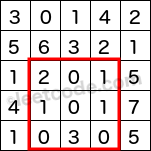
\includegraphics[width=150pt]{range.png}\\
\end{center}

\textbf{Example:}

\begin{Code}
Given matrix = [
  [3, 0, 1, 4, 2],
  [5, 6, 3, 2, 1],
  [1, 2, 0, 1, 5],
  [4, 1, 0, 1, 7],
  [1, 0, 3, 0, 5]
]

sumRegion(2, 1, 4, 3) -> 8
update(3, 2, 2)
sumRegion(2, 1, 4, 3) -> 10
\end{Code}

\textbf{Note:}

1. The matrix is only modifiable by the update function.

2. You may assume the number of calls to update and sumRegion function is distributed evenly.

3. You may assume that row1 ≤ row2 and col1 ≤ col2.

\subsubsection{Solution I}

\begin{Code}
public class NumMatrixII {
    private int m, n;

    private int[][] tree;
    private int[][] nums;

    public NumMatrixII(int[][] matrix) {
        if (matrix.length == 0 || matrix[0].length == 0) {
            return;
        }

        m = matrix.length;
        n = matrix[0].length;
        nums = new int[m][n];
        tree = new int[m + 1][n + 1];

        for (int i = 0; i < m; i++) {
            for (int j = 0; j < n; j++) {
                update(i, j, matrix[i][j]);
            }
        }
    }

    public void update(int row, int col, int val) {
        if (m == 0 || n == 0) {
            return;
        }
        int delta = val - nums[row][col];
        nums[row][col] = val;

        for (int i = row + 1; i <= m; i += i & (-i)) {
            for (int j = col + 1; j <= n; j += j & (-j)) {
                tree[i][j] += delta;
            }
        }
    }

    private int sum(int row, int col) {
        int sum = 0;
        for (int i = row + 1; i > 0; i -= i & (-i)) {
            for (int j = col + 1; j > 0; j -= j & (-j)) {
                sum += tree[i][j];
            }
        }
        return sum;
    }

    public int sumRegion(int row1, int col1, int row2, int col2) {
        if (m == 0 || n == 0) {
            return 0;
        }
        return sum(row2, col2) - sum(row2, col1 - 1) - sum(row1 - 1, col2) + sum(row1 - 1, col1 - 1);
    }
}
\end{Code}

\newpage

\subsubsection{Solution II}

\begin{Code}
public class NumMatrixII {
    private int[][] mMatrix;
    private int mRow, mCol;

    public NumMatrixII(int[][] matrix) {
        if (matrix.length == 0) {
            return;
        }

        mRow = matrix.length;
        mCol = matrix[0].length;

        for (int i = 0; i < mRow; i++) {
            for (int j = 0; j < mCol; j++) {
                matrix[i][j] += matrix[i][j - 1];
            }
        }
        mMatrix = matrix;
    }

    public void update(int row, int col, int val) {
        int orig = mMatrix[row][col] - (col > 0 ? mMatrix[row][col - 1] : 0);
        int delta = val - orig;
        for (int i = col; i < mCol; i++) {
            mMatrix[row][i] += delta;
        }
    }

    public int sumRegion(int row1, int col1, int row2, int col2) {
        int sum = 0;
        for (int i = row1; i <= row2; i++) {
            sum += mMatrix[i][col2] - (col1 > 0 ? mMatrix[i][col1 - 1] : 0);
        }
        return sum;
    }
}
\end{Code}

\newpage